% !TEX root = ../thesis.tex

\chapter{Kvantovy system}

Stupeň vývoja kvantových počítačov nateraz neumožnuje priamy prístup k
fyzickému stroju. Tieto prototypy sú veľmi veľké a prísne strážené v 
laboratóriách. Našťastie existujú nástroje, ktorými je umožnená práca aj 
obyčajným ľuďom. Jedným z najpoužívanejším nástrojom je IBM Quantum Experience. 

\section{IBM Quantum Experience}
IBM Quantum Experience (ďalej len IBM QX) je webová aplikácia, ktorá 
slúži na experimentovanie s kvantovým počítačom. Medzi jej funkcionality 
možno zahrnúť vytváranie a ukladanie kvantových obvodov ako aj ich 
vykonávanie na kvantovom počítači. Tento počítač je symulovaný virtuálny 
stroj, no IBM QX umožnuje aj odoslanie experimentu na reálny počítač. 
Symulátor umožnuje relatívne rýchlu prácu s kvantovým počítačom. Tento
prístup odľachčuje skutočný systém od veľkej sieťovej premávky a takisto 
zlepšuje používaťeľský zážitok.

Vytáranie nového obvodu je veľmi intuitívne. Na obrázku \ref{ibm_qx_composer}
je nástroj na to určený. Prednastavené hradlá je spôsobom ťahaj a pusť (angl.
drag and drop) možné presúvať na plán kvantového obvodu. Po uložení je možné
spustiť tento program. Na server sa odošle experiment, za predpokladu, že
je obvod spúšťaný na simulátore, tak za krátku dobu sú vrátené výsledky.

\begin{figure} 
	\centering 
	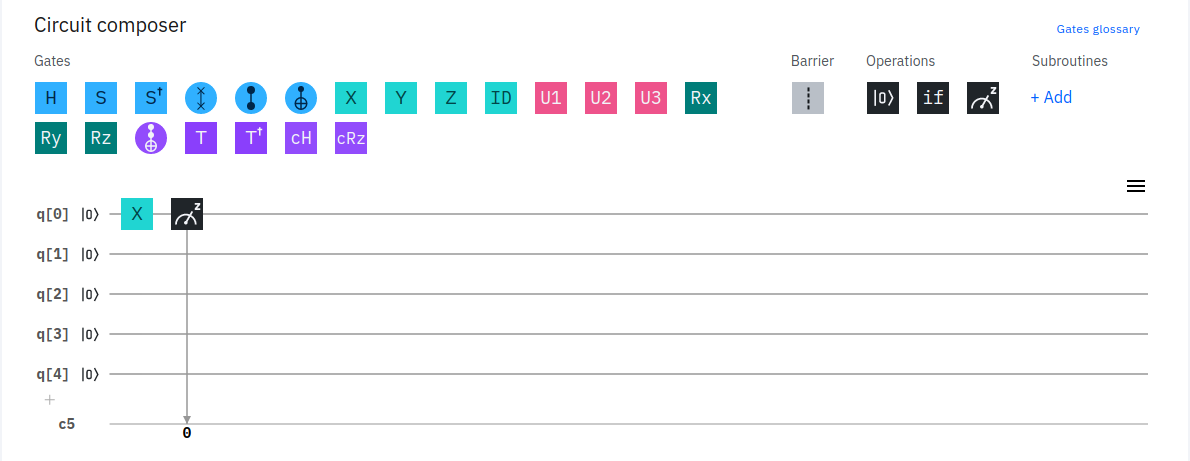
\includegraphics[width=1\textwidth]{figures/ibm_qx_composer.png} 
	\caption{Nástroj na tvorbu kvantových obvodov v IBM Quatnum Experience.}
    \label{ibm_qx_composer}
\end{figure}

Obvody je možné navrhovať aj pomocou špeciálneho jazyka podobného jazyku 
Python. Je samozrejmé, že IBM QX obsahuje aj editor pre tento jazyk.

\subsection{Stavy a ich zapis}
\subsection{Operacie kvantovych hradiel}
